\section{Managing different configurations}

\subsection{Objectives}

	\begin{frame}
		\frametitle{Objectives}
		
		Now that we have a worker in kubernetes, we want to be able to configure it.
		
		Also, we want to be able to differentiate between development and production configuration.
		
	\end{frame}
	
\subsection{Kustomize}	
	
	\begin{frame}
		\frametitle{Kustomize among other solutions}
		
		\begin{center}
		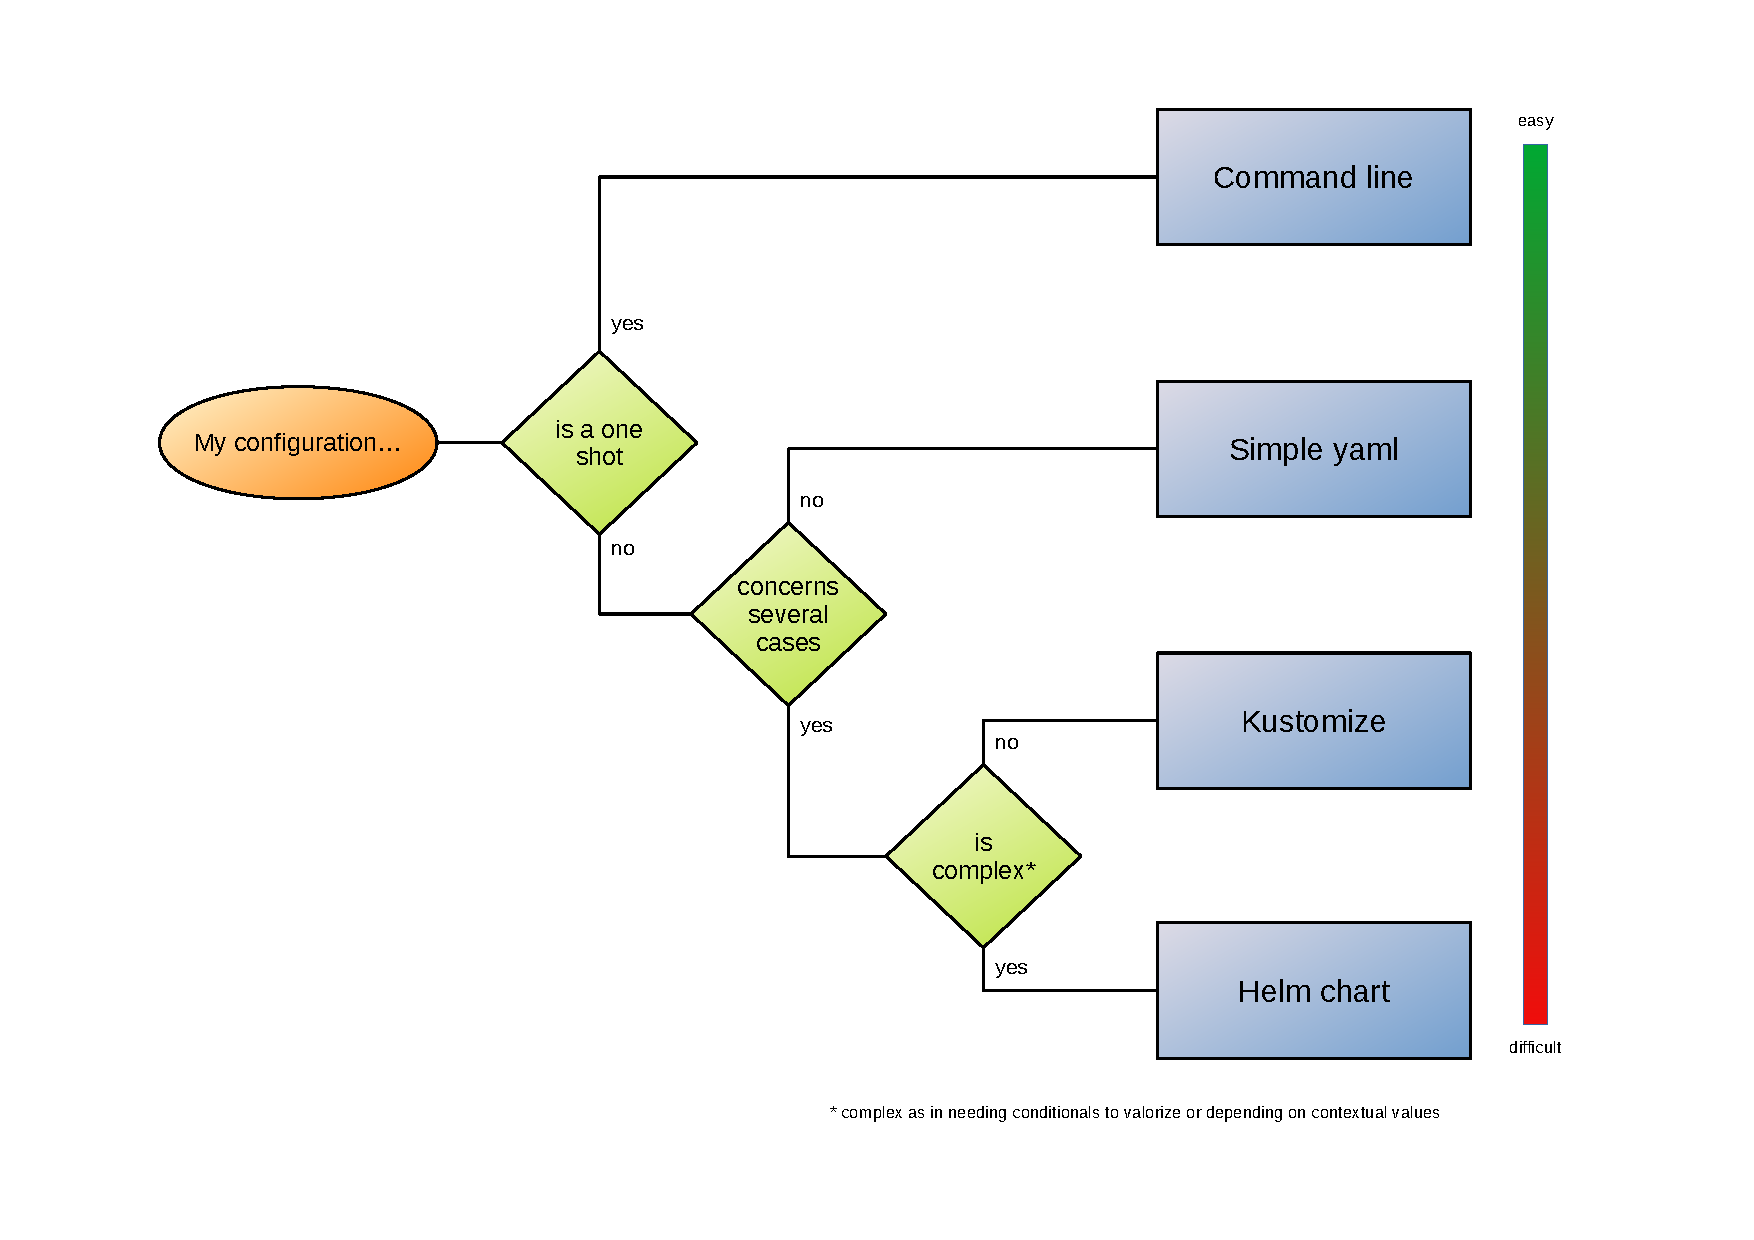
\includegraphics[height=7.5cm]{../../../resources/color/choiceConfigKind.pdf}
		\end{center}
	\end{frame}
	
	\begin{frame}
		\frametitle{Kustomize: a layered base configuration}
		
		\begin{center}
		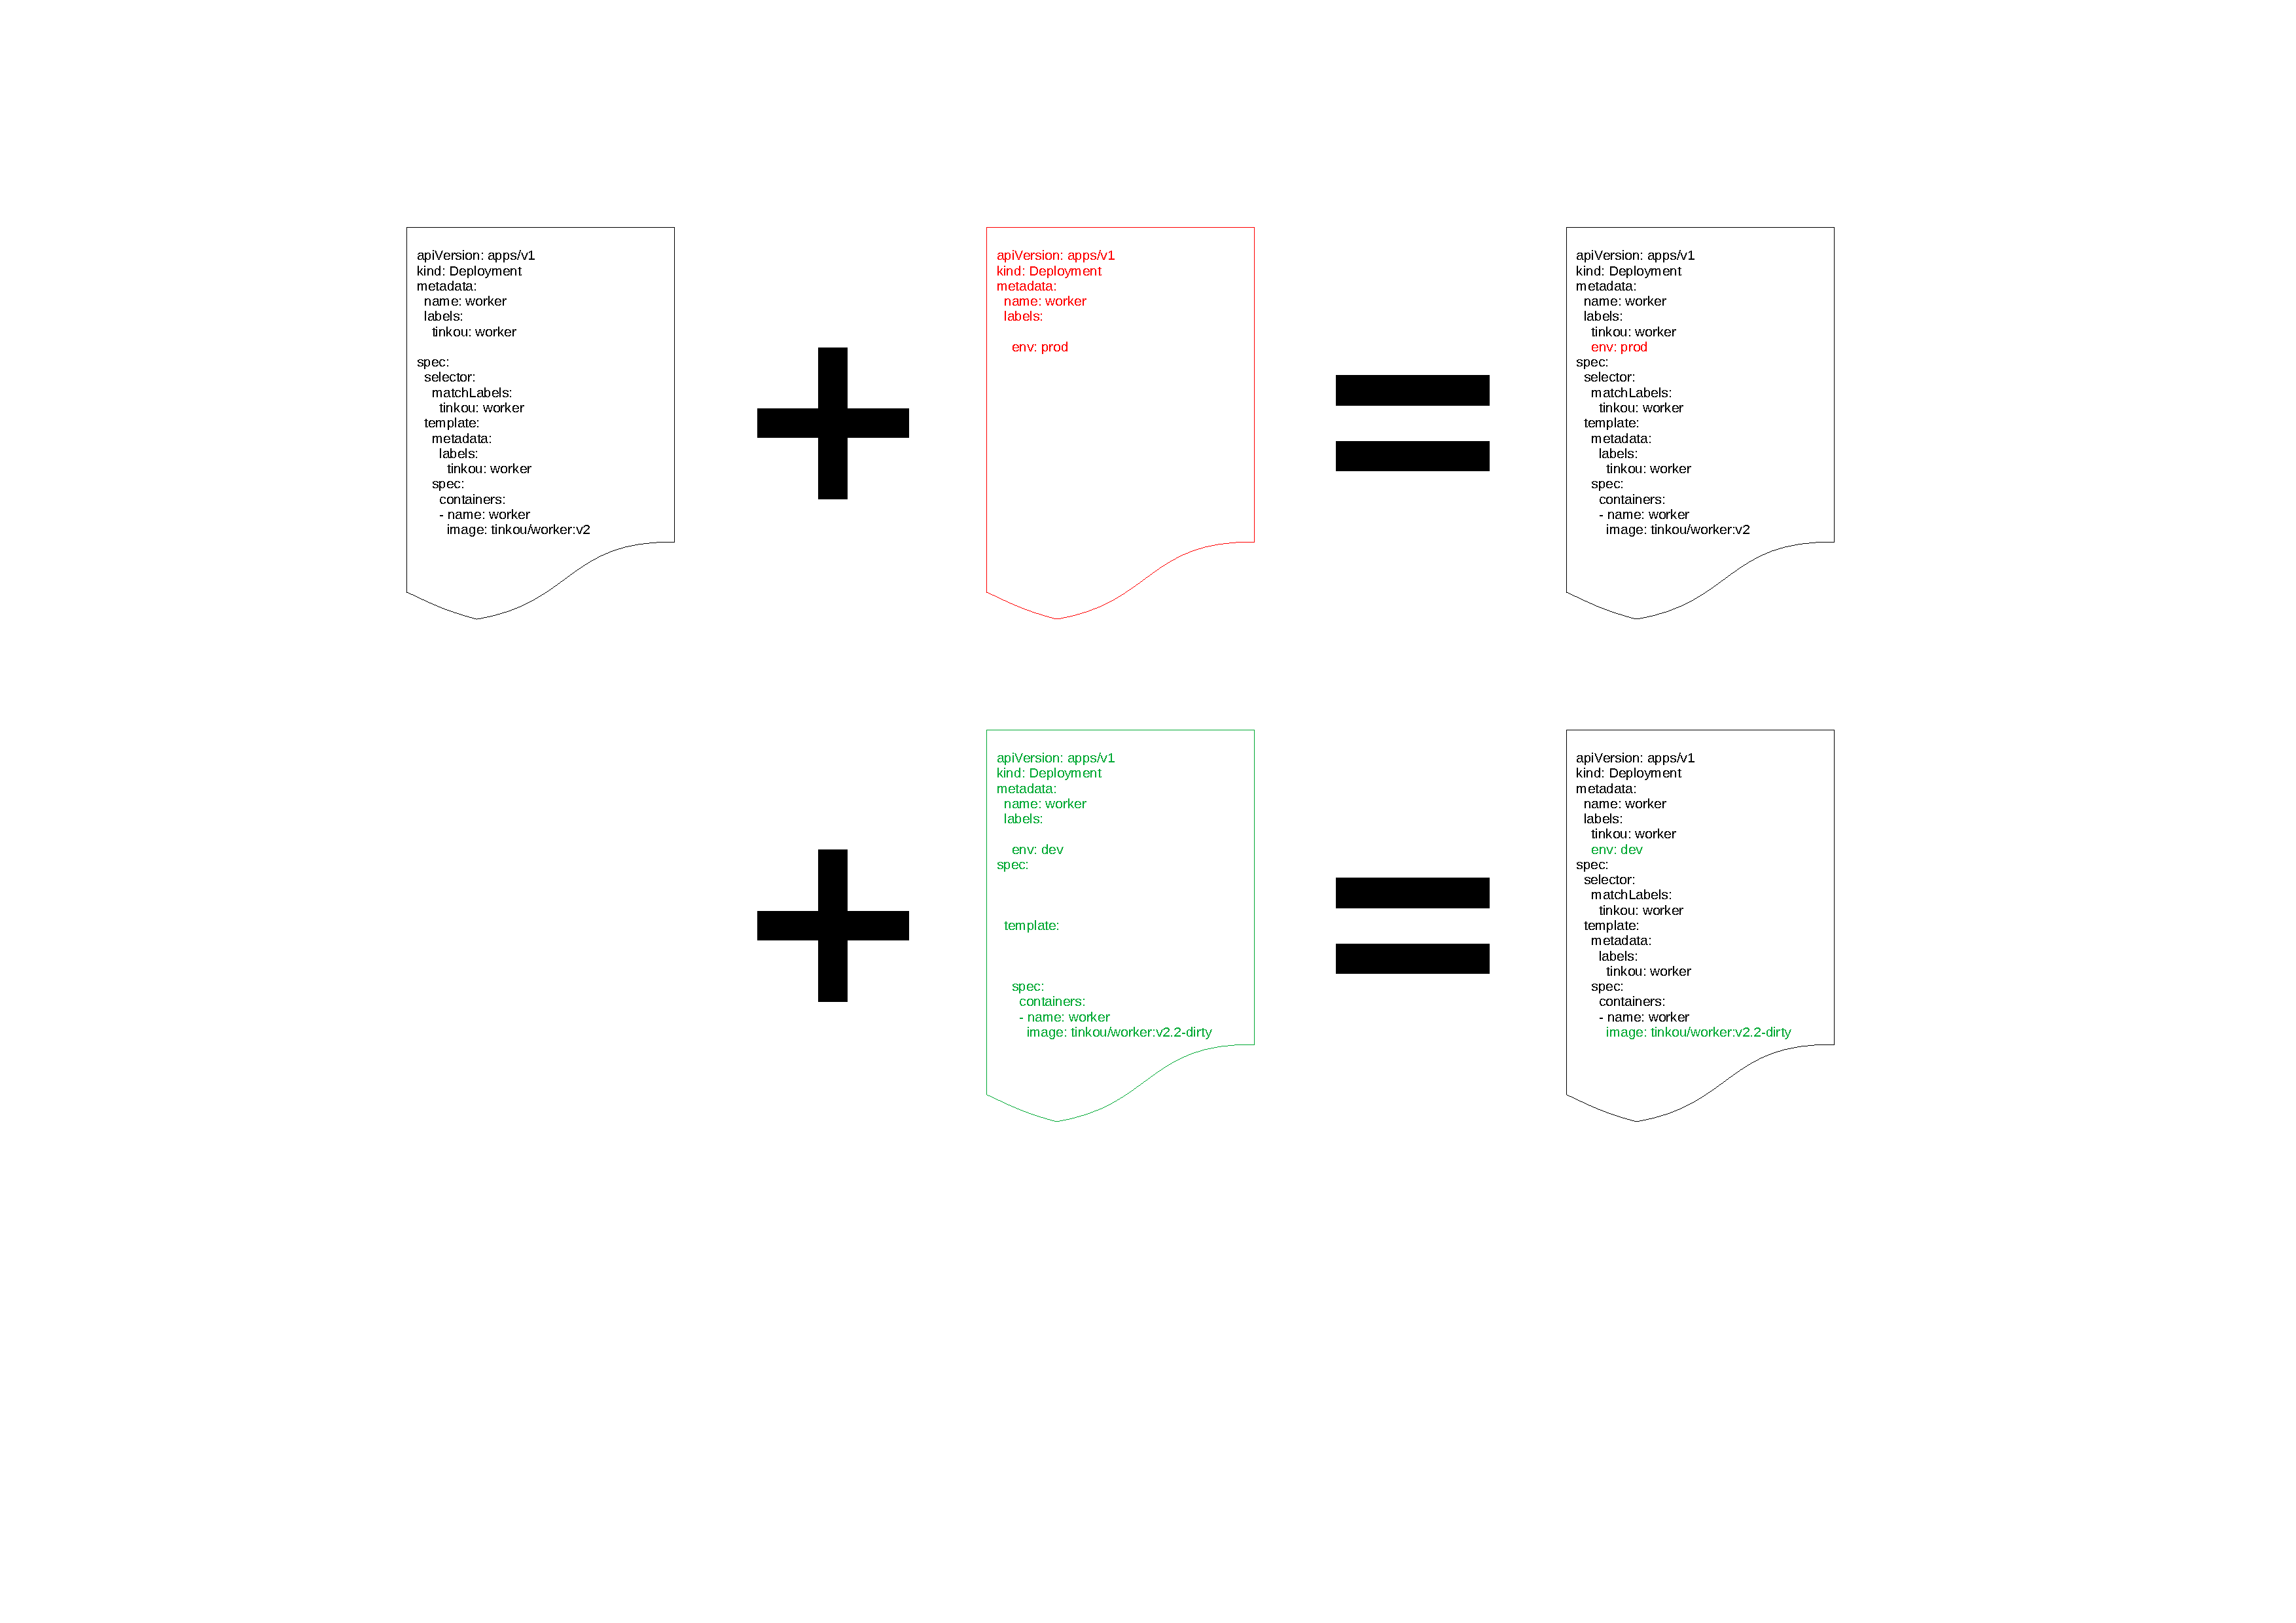
\includegraphics[height=7.5cm]{../../../resources/color/layeredConfiguration.pdf}
		\end{center}
	\end{frame}

\subsection{Using kustomize}	
	\begin{frame}[fragile]
		\frametitle{Initializing the base}
		
		We create a folder tree to sort our files
		\begin{block}{Command terminal in folder worker}
			\begin{verbatim}
				mkdir -p kube/base
				cd kube/base
			\end{verbatim}
		\end{block}
		
		\bigskip
		
		\begin{footnotesize}
			Logs terminal still had "\verb!stern worker!" running
			
			Monitor terminal still had "\verb!kubectl get pods -w!" running
		\end{footnotesize}
	\end{frame}
	
	\begin{frame}[fragile]
		\frametitle{Initializing the base}
		
		We are starting with a source.yaml file describing our deployment
		\begin{block}{worker/kube/base/source.yaml}
			\begin{tiny}
				\begin{verbatim}
					apiVersion: apps/v1
					kind: Deployment
					metadata:
					  name: worker
					  labels:
					    tinkou: worker
					spec:
					  selector:
					    matchLabels:
					      tinkou: worker
					  template:
					    metadata:
					      labels:
					        tinkou: worker
					    spec:
					      containers:
					      - name: worker
					        image: tinkou/worker:v1
				\end{verbatim}
			\end{tiny}
		\end{block}
	\end{frame}
	
	\begin{frame}[fragile]
		\frametitle{Initializing the base}
		\begin{block}{Command terminal in folder worker/kube/base}
			\begin{verbatim}
				kustomize create --autodetect
				kustomize build
				kubectl apply -k .
			\end{verbatim}
		\end{block}
	\end{frame}
	
	\begin{frame}[fragile]
		\frametitle{Initializing the base}
		As we modify an immutable field, we need to delete the previous deployment before:
		\begin{block}{Command terminal in folder worker/kube/base}
			\begin{verbatim}
				kubectl delete deployment worker
				kubectl apply -k .
			\end{verbatim}
		\end{block}
	\end{frame}
	
	\begin{frame}[fragile]
		\frametitle{Adding a parameter to our worker}
		
		Modify the worker to use a parameter:
		\begin{block}{worker/worker.sh}
			\begin{verbatim}
				#!/usr/bin/env bash
				while true; do
				  echo "I'm $NAME and it is $(date)"
				  sleep 2
				done
			\end{verbatim}
		\end{block}
	\end{frame}
	
	\begin{frame}[fragile]
		\frametitle{Deploying the new version in our cluster}
		
		First we create a new version of the image:
		\begin{block}{Command terminal in folder worker}
			\begin{verbatim}
				docker build -t tinkou/worker:v2 .
			\end{verbatim}
		\end{block}
	\end{frame}
	
	\begin{frame}[fragile]
		\frametitle{Deploying the new version in our cluster}
		
		Update source.yaml the field \verb!.spec.template.spec!:
		\begin{block}{worker/kube/base/source.yaml}
			\begin{tiny}
				\begin{verbatim}
					apiVersion: apps/v1
					kind: Deployment
					metadata:
					  name: worker
					  labels:
					    tinkou: worker
					spec:
					  selector:
					    matchLabels:
					      tinkou: worker
					  template:
					    metadata:
					      labels:
					        tinkou: worker
					    spec:
					      containers:
					      - name: worker
					        image: tinkou/worker:v2
					        env:
					        - name: NAME
					          value: Bink
				\end{verbatim}
			\end{tiny}
		\end{block}
	\end{frame}
	
	\begin{frame}[fragile]
		\frametitle{Deploying the new version in our cluster}
			
		And finally apply the modification:
		\begin{block}{Command terminal in folder worker}
			\begin{small}
					\begin{verbatim}
					kubectl apply -k kube/base
				\end{verbatim}
			\end{small}
		\end{block}
		
		\bigskip
		
		\visible<2->{
			To clean what has been deployed:
		}
		\begin{block}{Command terminal in folder worker}<2->
			\begin{verbatim}
				kubectl delete -k kube/base
			\end{verbatim}
		\end{block}
	\end{frame}
	
	\begin{frame}
		\frametitle{Deploying the new version in our cluster}
		
		There are too many operations.
		
		\bigskip
		Is there a way to simplify this?
	\end{frame}
	
\subsection{Using skaffold}	
	
	\begin{frame}
		\frametitle{Skaffold}
		
		Skaffold is a developer oriented tool created to simplify the packaging and deployment on kubernetes.
		
		\medskip
		The Skaffold documentation can be found \href{https://github.com/GoogleContainerTools/skaffold}{here}.

	\end{frame}
	
	\begin{frame}[fragile]
		\frametitle{Initializing skaffold}
		
		Let's initialize skaffold:
		\begin{block}{Command terminal in folder worker}
			\begin{verbatim}
				skaffold init
			\end{verbatim}
			Follow the application command line interface.
		\end{block}
	\end{frame}
	
	\begin{frame}[fragile]
		\frametitle{Initializing skaffold}

		Skaffold detects the yaml and skaffold.yaml needs to be configured to use kustomize:
		\begin{block}{worker/skaffold.yaml}
			\begin{footnotesize}
				\begin{verbatim}
					apiVersion: skaffold/v1beta15
					kind: Config
					metadata:
					  name: worker
					build:
					  artifacts:
					  - image: tinkou/worker
					deploy:
					  kustomize:
					    path: kube/base
				\end{verbatim}						
			\end{footnotesize}
		\end{block}
		The \verb!apiVersion! can change with skaffold version.
	\end{frame}
	
	\begin{frame}[fragile]
		\frametitle{Using Skaffold}
		
		Let's use Skaffold to build our image:
		\begin{block}{Command terminal in folder worker}
			\begin{verbatim}
				skaffold run
			\end{verbatim}
		\end{block}
		
		\bigskip
		
		\visible<2->{
			A particularity of Skaffold is that to work with minikube, the current context of kubectl must be "minikube".\\
			The current context can be with:
		}

		\begin{block}{Command terminal}<2->
			\begin{verbatim}
				kubectl config current-context
			\end{verbatim}
		\end{block}				
	\end{frame}
	
	\begin{frame}[fragile]
		\frametitle{Using skaffold}
		
		We are going to test a little skaffold commands:
		\begin{block}{Command terminal in folder worker}
			\begin{verbatim}
				skaffold build
				skaffold run
				skaffold delete
			\end{verbatim}					
		\end{block}
		
		\begin{description}
			\item[build] only build the image and push it in the registry (except in minikube)
			\item[run] build, push and run the image in kubectl current cluster
			\item[delete] delete run element from the kubectl current cluster
		\end{description}
	
	\end{frame}
	
	\begin{frame}[fragile]
		\frametitle{Using skaffold}
		
		Lets try the dev function:
		\begin{block}{Command terminal in folder worker}
			\begin{verbatim}
				skaffold dev
			\end{verbatim}					
		\end{block}

		It works like run, but displays logs and stays in foreground.
	\end{frame}
	
	\begin{frame}
		\frametitle{Using skaffold}

		Open a command line in a new window 4.		
		
		Try to modify the file worker.sh in this new command line.
		
		\bigskip
		
		And look at how skaffold dynamically builds and deploys each time the file is saved.
	\end{frame}
	
	\begin{frame}[fragile]
		\frametitle{Isolating the configuration in a configmap}

		Add a file conf.env in the folder base:
		\begin{block}{worker/kube/base/conf.env}
			\begin{verbatim}
				NAME=Trent
			\end{verbatim}
		\end{block}				
		
		\begin{block}{Second command terminal in the folder worker/kube/base}
			\begin{verbatim}
				kustomize edit add configmap worker \
				                   --from-env-file conf.env
			\end{verbatim}
		\end{block}
	\end{frame}

	\begin{frame}[fragile]
		\frametitle{Isolating the configuration in a configmap}

		\begin{block}{worker/kube/base/source.yaml}
			\begin{tiny}
				\begin{verbatim}
					apiVersion: apps/v1
					kind: Deployment
					metadata:
					  name: worker
					  labels:
					    tinkou: worker
					spec:
					  selector:
					    matchLabels:
					      tinkou: worker
					  template:
					    metadata:
					      labels:
					        tinkou: worker
					    spec:
					      containers:
					      - name: worker
					        image: tinkou/worker:v2
					        envFrom:
					        - configMapRef:
					            name: worker
				\end{verbatim}
			\end{tiny}			
		\end{block}
	\end{frame}
	
	\begin{frame}[fragile]
		\frametitle{Defining a local configuration}
		
		Create a folder \verb!worker/kube/local!, and add in it the file \verb!patch.yaml!:
		\begin{block}{worker/kube/local/patch.yaml}
			\begin{verbatim}
				apiVersion: v1
				kind: ConfigMap
				metadata:
				  name: worker
				data:
				  NAME: Iris
			\end{verbatim}
		\end{block}
		
		\medskip
		
		\visible<2->{
			Nothing happens in skaffold dev.
		}
	\end{frame}
	
	\begin{frame}[fragile]
		\frametitle{Defining a local configuration: kustomize}
		
		First create a new kustomize project with a base resource and the patch:
		\begin{block}{Second command terminal in folder worker/kube/local}
			\begin{verbatim}
				kustomize create --resources ../base
				kustomize edit add patch patch.yaml
			\end{verbatim}
		\end{block}
		
		\visible<2->{
			Still nothing in skaffold dev.
		}
	\end{frame}
	
	\begin{frame}[fragile]
		\frametitle{Defining a local configuration: skaffold}
		
		Indicate to skaffold to use this local values when using minikube:
		\begin{block}{worker/skaffold.yaml}
			\begin{tiny}
				\begin{verbatim}
						apiVersion: skaffold/v1beta15
						kind: Config
						metadata:
						  name: worker
						build:
						  artifacts:
						  - image: tinkou/worker
						deploy:
						  kustomize:
						    path: kube/base
						profiles:
						- name: local
						  activation:
						  - kubeContext: minikube
						  deploy:
						    kustomize:
						      path: /kube/local
				\end{verbatim}
			\end{tiny}
		\end{block}
	
	\end{frame}
	
	\begin{frame}[fragile]
		\frametitle{Using skaffold dev modifications detection}
		
		Now the modification is deployed.
		
		Lets modify the base configuration:
		\begin{block}{worker/kube/base/conf.env}
			\begin{verbatim}
				NAME=Dor
			\end{verbatim}
		\end{block}
		
		\visible<2->{
			Skaffold do not react.
			
			\medskip
			
			Try to modify several files to see how skaffold detection works.
		}
	\end{frame}
	
	\begin{frame}[fragile]
		\frametitle{Cleaning up}
		
		If you kill the command \verb!skaffold dev! with \textbf{Ctrl+C}, skaffold will clean what it has deployed.
	\end{frame}
	
	\begin{frame}
		\begin{center}
			Questions?
		\end{center}
	\end{frame}